% ============================================================
%  CHAPITRE 2 — ANALYSE ET CONCEPTION
% ============================================================
\chapter{Analyse et Conception}
\label{chap:conception}

\section{Introduction}

Après l'étude bibliographique présentée au chapitre précédent, ce chapitre est consacré à l'analyse fonctionnelle et à la conception de la solution proposée. Il s'agit de définir précisément les besoins du système, les exigences attendues ainsi que l'architecture technique retenue pour la mise en œuvre. À cette fin, nous analysons tout d'abord les besoins et contraintes du drone lors d'un scénario de secours.

\section{Analyse du besoin et exigences du système}
\label{sec:analyse-besoin}

Le besoin principal du projet est de permettre à un drone autonome d'identifier automatiquement une zone d'atterrissage sécurisée lors d'une situation critique, en minimisant les risques de collision. Le système doit collecter les données visuelles, analyser l'environnement, détecter les obstacles et générer une décision d'atterrissage en temps quasi réel.

L'acteur principal identifié est l'opérateur du drone, qui déclenche la mission et la surveille, tandis que le système autonome exécute automatiquement la capture d'image, la segmentation, la détection d'obstacles, la sélection de la zone sûre et la décision d'atterrissage.

À partir de cette analyse, les exigences du système ont été regroupées en exigences fonctionnelles et non fonctionnelles :

\begin{table}[!ht]
  \centering
  \caption{Exigences fonctionnelles du système.}
  \label{tab:exigences-fonct}
  \renewcommand{\arraystretch}{1.4}
  \begin{tabularx}{0.85\textwidth}{
    >{\bfseries\color{ENIADBlue}}c
    >{\centering\arraybackslash}X
    >{\centering\arraybackslash}c
  }
    \toprule
    \rowcolor{ENIADBlue!12}
    \textbf{ID} & \textbf{Exigence fonctionnelle} & \textbf{Priorité} \\
    \midrule
    F1 & Capturer l'image & Haute \\
    \rowcolor{ENIADLightBlue!20}
    F2 & Segmenter l'image & Haute \\
    F3 & Détecter les obstacles & Haute \\
    \rowcolor{ENIADLightBlue!20}
    F4 & Calculer la zone sûre & Haute \\
    F5 & Retourner la décision & Haute \\
    \bottomrule
  \end{tabularx}
\end{table}

\begin{table}[!ht]
  \centering
  \caption{Exigences non fonctionnelles du système.}
  \label{tab:exigences-nonfonct}
  \renewcommand{\arraystretch}{1.4}
  \begin{tabularx}{0.85\textwidth}{
    >{\bfseries\color{ENIADBlue}}c
    >{\centering\arraybackslash}X
    >{\centering\arraybackslash}c
  }
    \toprule
    \rowcolor{ENIADBlue!12}
    \textbf{ID} & \textbf{Exigence non fonctionnelle} & \textbf{Valeur cible} \\
    \midrule
    NF1 & Temps d'inférence & $<$ 100 ms \\
    \rowcolor{ENIADLightBlue!20}
    NF2 & Débit de traitement & FPS $>$ 15 \\
    NF3 & Disponibilité & $>$ 95~\% \\
    \rowcolor{ENIADLightBlue!20}
    NF4 & Consommation énergétique & Réduite \\
    NF5 & Évolutivité & Architecture modulaire \\
    \bottomrule
  \end{tabularx}
\end{table}

Ces exigences permettent de structurer la conception globale du système et la répartition de ses modules, présentée dans la section suivante.

\section{Architecture globale et conception technique}
\label{sec:architecture}

Le système est organisé sous forme d'un pipeline intelligent assurant une exécution continue depuis l'acquisition de l'image jusqu'à la décision d'atterrissage :

\begin{center}
  \textbf{Drone} $\rightarrow$ \textbf{Caméra} $\rightarrow$ \textbf{Prétraitement} $\rightarrow$ \textbf{Segmentation U-Net} $\rightarrow$ \textbf{Analyse des zones} $\rightarrow$ \textbf{Décision} $\rightarrow$ \textbf{Atterrissage}
\end{center}

La caméra constitue la source principale d'information, tandis que le modèle de segmentation représente le cœur décisionnel du système. Sur le plan logiciel, la solution est organisée en modules indépendants — gestion du dataset, entraînement, inférence, exécution Edge, API et visualisation — facilitant la maintenance, l'évolutivité et la réutilisation du code.

\subsection{Diagramme de séquence}
\label{sec:sequence-diag}

Le diagramme de séquence (figure~\ref{fig:sequence-diag}) modélise le flux temporel détaillé des messages échangés entre les entités matérielles et logicielles lors de l'évacuation de sécurité. Le scénario débute par le déclenchement du mode urgence de l'aéronef vers l'interface de contrôle et l'acquisition d'images par la caméra vers la Raspberry Pi 4. Cette dernière sollicite le module de décision qui appelle l'inférence du modèle de segmentation Attention U-Net. Un bloc d'itération (\textit{loop}) calcule alors le point d'atterrissage optimal via l'analyse des zones sûres (recherche des composantes connexes, sélection de la plus grande aire, application de la Distance Transform et validation de la cible). Les coordonnées obtenues alimentent le module Guidance Controller (calcul des écarts $dx$, $dy$, distance et angle de gisement) et font transiter la Flight State Machine à travers les états SEARCHING, GUIDING et LANDING. Le Flight Controller génère ensuite les trajectoires de translation et de descente, transmises au pilote automatique PX4 via le protocole MAVLink (liaison Offboard). Enfin, la boucle de contrôle interne de l'autopilote PX4 (Position, Attitude et Motor Controllers) assure l'atterrissage autonome.

\begin{figure}[!ht]
  \centering
  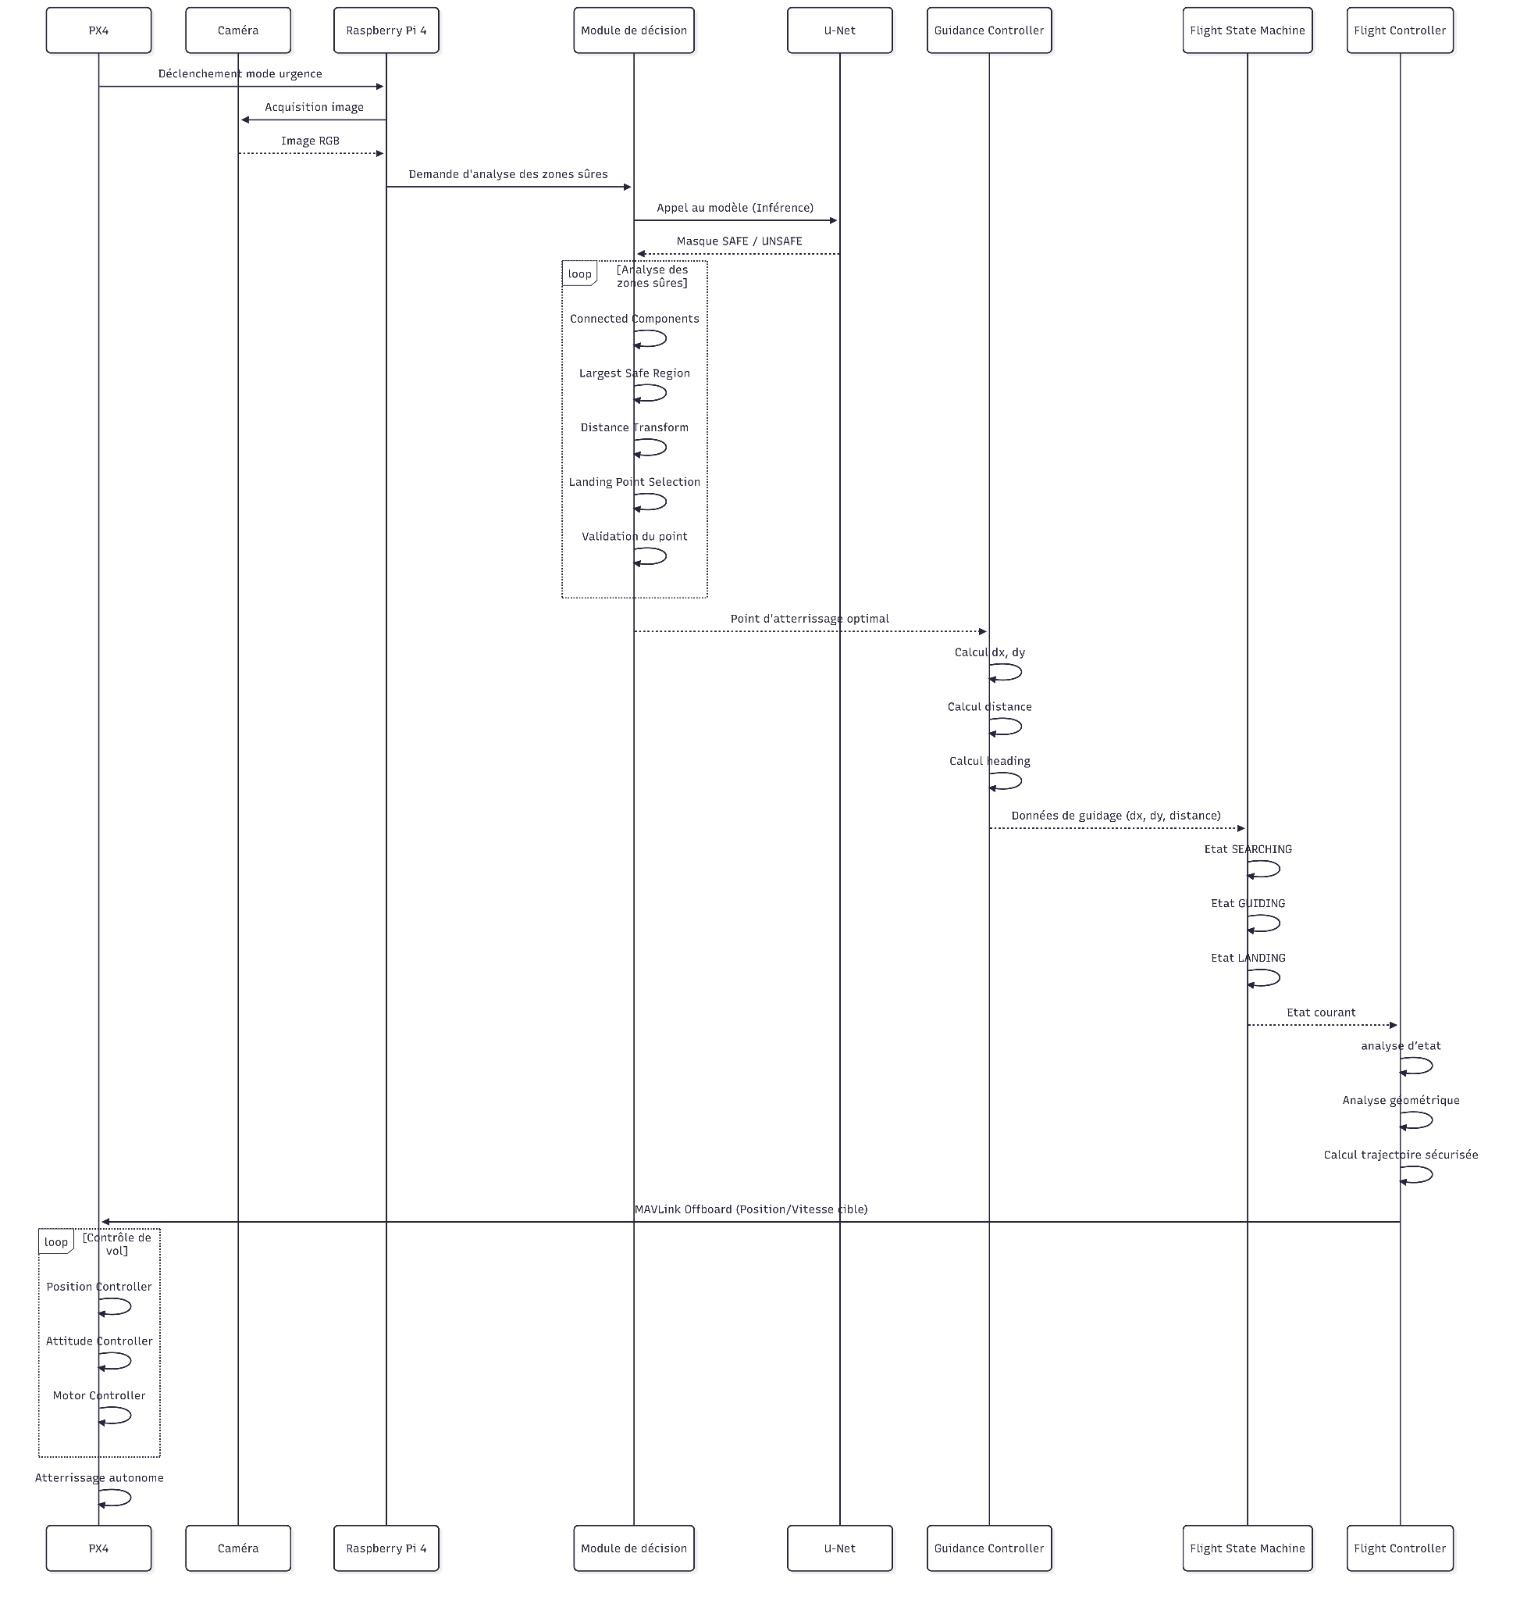
\includegraphics[width=0.7\textwidth,keepaspectratio]{assets/diagrams/sequ.jpeg}
  \caption{Flux temporel des messages entre les composants du système, incluant l'analyse des zones sûres, le calcul de guidage, la machine d'états de vol et le contrôle de vol via MAVLink.}
  \label{fig:sequence-diag}
\end{figure}

\subsection{Diagramme de composants}
\label{sec:components-diag}

Le diagramme de composants (figure~\ref{fig:components-diag}) présente l'architecture matérielle et logicielle modulaire du système global de descente d'urgence (\textit{Drone Autonomous Emergency Landing System}). L'ordinateur compagnon Raspberry Pi 4 héberge le module de vision (\textit{Vision Module}) assurant la capture caméra RGB et l'inférence par segmentation Attention U-Net. Il exécute également le module de décision (\textit{Emergency Landing System}) regroupant l'analyse des aires sûres, la sélection du point cible, le Guidance Controller, la Flight State Machine, le Flight Controller et la couche de communication avec le protocole MAVLink. En parallèle, l'autopilote PX4 intègre le module de surveillance (\textit{Monitoring Module}) alimenté par les capteurs embarqués (GPS, IMU, Baromètre), ainsi que les contrôleurs d'exécution bas niveau (Position Controller, Attitude Controller et Motor Controller) agissant sur la motorisation physique. Pour matérialiser cette conception modulaire, des choix d'outils et de technologies précis ont été retenus ; nous les détaillons dans la section suivante.

\begin{figure}[!hb]
  \centering
  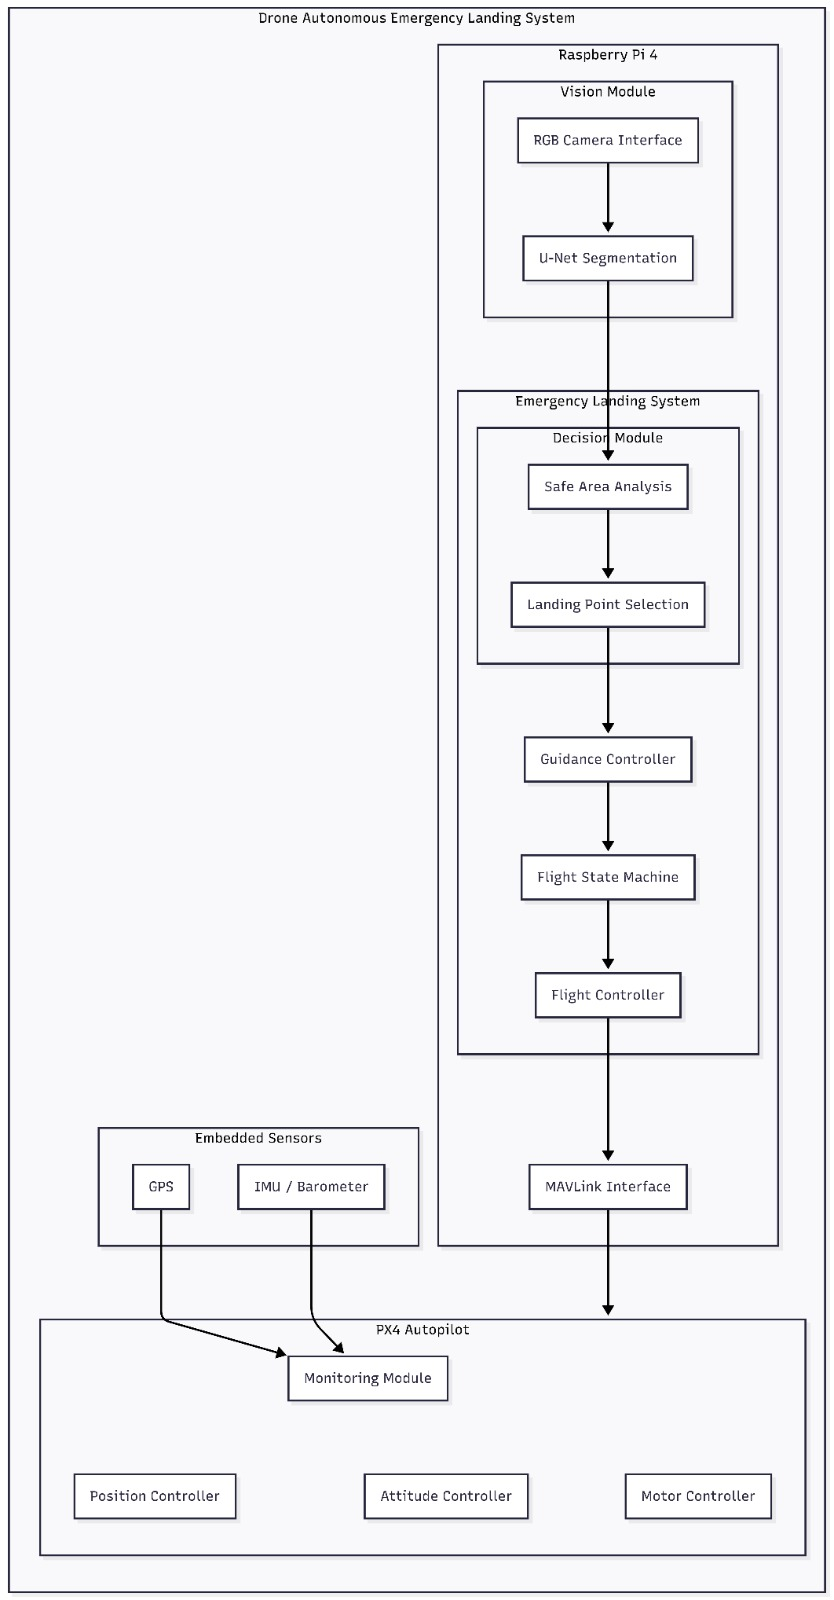
\includegraphics[width=0.55\textwidth,keepaspectratio]{assets/diagrams/compo.jpeg}
  \caption{Architecture logicielle et matérielle du système : modules de vision, de décision, de guidage et de contrôle de vol interfacés avec l'autopilote PX4 via MAVLink.}
  \label{fig:components-diag}
\end{figure}

\section{Outils et choix technologiques}
\label{sec:choix-tech}

La sélection des outils a été guidée par des critères de compatibilité, de performance, de support communautaire et de facilité de déploiement embarqué :

\vspace{0.8em}

\begin{tcolorbox}[colback=ENIADBlue!3, colframe=ENIADBlue!15, arc=4pt, boxrule=0.5pt, left=10pt, right=10pt, top=8pt, bottom=8pt]
  \begin{minipage}[c]{0.12\textwidth}
    \centering
    
\includegraphics[width=1.3cm,keepaspectratio]{images/logos/python.png}
  \end{minipage}
  \hfill
  \begin{minipage}[c]{0.84\textwidth}
    \textbf{\large Python} \\
    \textbf{Définition} : Langage de programmation dynamique de haut niveau, réputé pour sa flexibilité et la richesse de son écosystème scientifique. \\
    \textbf{Alternative} : C++ \\
    \textbf{Justification} : Retenu pour la rapidité de prototypage qu'il procure, la richesse de son écosystème de Data Science et la simplicité d'écriture des pipelines d'entraînement, bien que les modules critiques puissent être compilés par la suite pour le déploiement.
  \end{minipage}
\end{tcolorbox}

\begin{tcolorbox}[colback=ENIADBlue!3, colframe=ENIADBlue!15, arc=4pt, boxrule=0.5pt, left=10pt, right=10pt, top=8pt, bottom=8pt]
  \begin{minipage}[c]{0.12\textwidth}
    \centering
    
\includegraphics[width=1.3cm,keepaspectratio]{images/logos/pytorch.png}
  \end{minipage}
  \hfill
  \begin{minipage}[c]{0.84\textwidth}
    \textbf{\large PyTorch} \\
    \textbf{Définition} : Framework d'apprentissage profond open-source développé par Meta AI, facilitant la création et l'entraînement de réseaux de neurones. \\
    \textbf{Alternative} : TensorFlow \\
    \textbf{Justification} : Préféré pour sa conception intuitive basée sur des graphes de calcul dynamiques, simplifiant grandement le débogage et l'expérimentation rapide de l'architecture.
  \end{minipage}
\end{tcolorbox}

\begin{tcolorbox}[colback=ENIADBlue!3, colframe=ENIADBlue!15, arc=4pt, boxrule=0.5pt, left=10pt, right=10pt, top=8pt, bottom=8pt]
  \begin{minipage}[c]{0.12\textwidth}
    \centering
    
\includegraphics[width=1.3cm,keepaspectratio]{images/logos/opencv.png}
  \end{minipage}
  \hfill
  \begin{minipage}[c]{0.84\textwidth}
    \textbf{\large OpenCV} \\
    \textbf{Définition} : Bibliothèque open-source de vision par ordinateur optimisée pour le traitement d'images et la vidéo en temps réel. \\
    \textbf{Alternative} : PIL (Pillow) \\
    \textbf{Justification} : S'impose grâce à ses algorithmes natifs optimisés en C++, sa gestion des formats de caméras industrielles et sa compatibilité directe avec les tenseurs de PyTorch.
  \end{minipage}
\end{tcolorbox}

\begin{tcolorbox}[colback=ENIADBlue!3, colframe=ENIADBlue!15, arc=4pt, boxrule=0.5pt, left=10pt, right=10pt, top=8pt, bottom=8pt]
  \begin{minipage}[c]{0.12\textwidth}
    \centering
    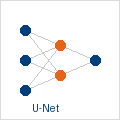
\includegraphics[width=1.3cm,keepaspectratio]{images/logos/unet.png}
  \end{minipage}
  \hfill
  \begin{minipage}[c]{0.84\textwidth}
    \textbf{\large U-Net} \\
    \textbf{Définition} : Architecture de réseau neuronal convolutif symétrique doté de skip connections, dédié à la segmentation d'images. \\
    \textbf{Alternative} : DeepLab \\
    \textbf{Justification} : Privilégié pour sa légèreté inhérente adaptée à l'Edge AI et sa capacité à préserver les frontières fines de segmentation avec un jeu de données réduit.
  \end{minipage}
\end{tcolorbox}

\begin{tcolorbox}[colback=ENIADBlue!3, colframe=ENIADBlue!15, arc=4pt, boxrule=0.5pt, left=10pt, right=10pt, top=8pt, bottom=8pt]
  \begin{minipage}[c]{0.12\textwidth}
    \centering
    
\includegraphics[width=1.3cm,keepaspectratio]{images/logos/onnx.png}
  \end{minipage}
  \hfill
  \begin{minipage}[c]{0.84\textwidth}
    \textbf{\large ONNX} \\
    \textbf{Définition} : Format ouvert et standard d'échange de modèles de Deep Learning favorisant l'interopérabilité entre outils et frameworks. \\
    \textbf{Alternative} : TorchScript \\
    \textbf{Justification} : Retenu comme format d'échange universel, permettant d'exporter et de déployer le modèle sur des cibles matérielles hétérogènes sans dépendre de l'environnement PyTorch complet.
  \end{minipage}
\end{tcolorbox}

\begin{tcolorbox}[colback=ENIADBlue!3, colframe=ENIADBlue!15, arc=4pt, boxrule=0.5pt, left=10pt, right=10pt, top=8pt, bottom=8pt]
  \begin{minipage}[c]{0.12\textwidth}
    \centering
    
\includegraphics[width=1.3cm,keepaspectratio]{images/logos/tensorrt.png}
  \end{minipage}
  \hfill
  \begin{minipage}[c]{0.84\textwidth}
    \textbf{\large TensorRT} \\
    \textbf{Définition} : Kit de développement logiciel de NVIDIA optimisant les modèles pour l'inférence hautes performances sur processeur graphique. \\
    \textbf{Alternative} : OpenVINO \\
    \textbf{Justification} : Choisi car notre cible matérielle finale repose sur l'architecture NVIDIA (ex. Jetson Orin), garantissant des accélérations d'inférence maximales grâce à une compilation matérielle spécifique.
  \end{minipage}
\end{tcolorbox}

\begin{tcolorbox}[colback=ENIADBlue!3, colframe=ENIADBlue!15, arc=4pt, boxrule=0.5pt, left=10pt, right=10pt, top=8pt, bottom=8pt]
  \begin{minipage}[c]{0.12\textwidth}
    \centering
    
\includegraphics[width=1.3cm,keepaspectratio]{images/logos/cuda.png}
  \end{minipage}
  \hfill
  \begin{minipage}[c]{0.84\textwidth}
    \textbf{\large CUDA} \\
    \textbf{Définition} : Architecture de calcul parallèle et API développée par NVIDIA pour accélérer les traitements intensifs sur GPU. \\
    \textbf{Alternative} : CPU \\
    \textbf{Justification} : Indispensable pour la parallélisation massive des calculs matriciels du réseau, permettant d'inférer 10 fois plus vite et de satisfaire les impératifs du temps réel requis pour le guidage.
  \end{minipage}
\end{tcolorbox}

\subsection{Écosystème matériel et protocoles pour l'intégration drone}
\label{subsec:ecosysteme-drone}

Bien que l'implémentation actuelle de ce projet ait été réalisée et validée de manière logicielle et hors ligne (sans tests physiques sur machine volante), l'intégration réelle du système sur un vecteur aérien autonome implique un écosystème spécifique d'outils matériels et de protocoles de communication. Les fiches suivantes détaillent ces composants clés pour un futur déploiement embarqué :

\vspace{0.8em}

\begin{tcolorbox}[colback=ENIADBlue!3, colframe=ENIADBlue!15, arc=4pt, boxrule=0.5pt, left=10pt, right=10pt, top=8pt, bottom=8pt]
  \begin{minipage}[c]{0.12\textwidth}
    \centering
    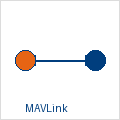
\includegraphics[width=1.3cm,keepaspectratio]{images/logos/mavlink.png}
  \end{minipage}
  \hfill
  \begin{minipage}[c]{0.84\textwidth}
    \textbf{\large MAVLink} \\
    \textbf{Définition} : Protocole de communication binaire léger sous forme de sérialisation de messages, conçu pour l'échange d'informations entre un pilote automatique et des composants embarqués ou stations sol. \\
    \textbf{Utilité potentielle} : Permettrait de transmettre en temps réel les coordonnées du point d'atterrissage optimal calculées par le module de vision vers l'autopilote et de récupérer la télémétrie du drone (altitude, attitude). \\
    \textbf{Statut d'utilisation} : \textbf{Non intégré / Non utilisé} dans l'implémentation physique actuelle de ce projet, constituant une perspective d'intégration matérielle.
  \end{minipage}
\end{tcolorbox}

\begin{tcolorbox}[colback=ENIADBlue!3, colframe=ENIADBlue!15, arc=4pt, boxrule=0.5pt, left=10pt, right=10pt, top=8pt, bottom=8pt]
  \begin{minipage}[c]{0.12\textwidth}
    \centering
    
\includegraphics[width=1.3cm,keepaspectratio]{images/logos/raspberrypi.png}
  \end{minipage}
  \hfill
  \begin{minipage}[c]{0.84\textwidth}
    \textbf{\large Raspberry Pi} \\
    \textbf{Définition} : Ordinateur monocarte à basse consommation d'énergie fonctionnant sous Linux, fréquemment configuré comme calculateur compagnon à bord du drone. \\
    \textbf{Utilité potentielle} : Servirait d'unité d'acquisition d'images de la caméra et de traitement d'inférence sémantique légère avant de piloter le contrôleur de vol principal via liaison série. \\
    \textbf{Statut d'utilisation} : \textbf{Non intégré / Non utilisé} dans l'implémentation physique actuelle de ce projet, les calculs ayant été validés hors ligne sur GPU de développement.
  \end{minipage}
\end{tcolorbox}

\begin{tcolorbox}[colback=ENIADBlue!3, colframe=ENIADBlue!15, arc=4pt, boxrule=0.5pt, left=10pt, right=10pt, top=8pt, bottom=8pt]
  \begin{minipage}[c]{0.12\textwidth}
    \centering
    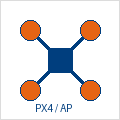
\includegraphics[width=1.3cm,keepaspectratio]{images/logos/px4.png}
  \end{minipage}
  \hfill
  \begin{minipage}[c]{0.84\textwidth}
    \textbf{\large PX4 / ArduPilot} \\
    \textbf{Définition} : Logiciels de contrôle de vol (\textit{firmwares}) de référence pour pilotes automatiques, assurant la stabilisation physique, le suivi de trajectoire et l'évitement d'obstacles bas niveau. \\
    \textbf{Utilité potentielle} : Géreraient la dynamique physique de vol et exécuteraient la commande de descente ou d'évitement reçue du compagnon de calcul IA via des ordres standardisés. \\
    \textbf{Statut d'utilisation} : \textbf{Non intégré / Non utilisé} dans l'implémentation physique actuelle de ce projet, le guidage ayant été modélisé de façon logicielle dans le notebook.
  \end{minipage}
\end{tcolorbox}

\vspace{0.8em}

Ces choix et perspectives offrent un compromis équilibré entre performance, précision et simplicité de déploiement, posant les bases techniques détaillées dans les chapitres suivants.

\vspace{1.5em}
\textbf{Conclusion}

En conclusion, ce deuxième chapitre a permis de traduire la problématique globale du projet en exigences fonctionnelles et non fonctionnelles concrètes. La modélisation de l'architecture par les diagrammes de séquence et de composants, conjuguée à la justification minutieuse de nos choix technologiques (Python, PyTorch, OpenCV, ONNX), a permis de définir une solution modulaire et optimale pour un environnement embarqué GPU. Fort de cette conception logicielle et matérielle validée, le chapitre suivant se penchera sur la mise en œuvre pratique en décrivant la préparation des données, le pipeline d'augmentation, et les étapes clés du développement de notre modèle de segmentation profonde.


\clearpage
